\documentclass[11pt]{article}

\usepackage{amsmath}
\usepackage[a4paper, margin=0.5in]{geometry}
\usepackage{graphicx} % daj an 1in jak chcesz normalniejszy margines, ale kod mi się w linii nie mieści :P
\usepackage[utf8]{inputenc}
\usepackage[T1]{fontenc}
\usepackage[polish]{babel}
\usepackage{float}
\usepackage{hyperref}
\usepackage{cleveref}
\usepackage{subfigure}

\title{Zadanie 5. Hybrydowy Algorytm Ewolucyjny}
\author{Oskar Kiliańczyk 151863 \& Wojciech Kot 151879}
\date{}

\begin{document}

\maketitle
\newpage

\section{Opis zadania}\label{sec:opis-zadania}

Celem zadania jest porównanie hybrydowego algorytmu z  i porównanie go z metodami
MSLS, ILS i LNS z poprzedniego zadania.
Opisy tych metod znajdują się w poprzednim sprawozdaniu.

\section{Opisy algorytmów}\label{sec:opisy-alg}

\subsection{Hybrydowy Algorytm Ewolucyjny}\label{subsec:hybrydowy-algorytm-ewolucyjny}
\begin{itemize}
    \item steady state
    \item z populacją elitarną 20 osobników
    \item Usuwanie duplikatów rozwiązań (Dwa rozwiązania są uznawane za duplikat, jeśli mają identyczną wartość funkcji celu)
    \item Wykorzystywane parametry to flagi use\_mutation, use\_local\_search oraz mutation\_rate = 0.1
\end{itemize}


\subsubsection{Główny algorytm}
\begin{enumerate}
    \item Wygeneruj populację początkową.
    \item Dopóki czas nie został przekroczony, powtarzaj:
    \begin{enumerate}
        \item Wybierz parę rodziców (rodzic1, rodzic2) losowo z populacji
        \item Utwórz dwa rozwiązania potomne* (Procedura rekombinacji)
        \item Jeśli jest ustawiona flaga use\_mutation - wykonaj mutację** (Procedura mutacji)
        \item Jeśli jest ustawiona flaga use\_local\_search - wykonaj przeszukiwanie lokalne
        \item Oblicz koszt rozwiązań potomnych
        \item Dla każdego z rozwiązań potomnych:
        \begin{enumerate}
            \item Jeśli koszt rozwiązania potomnego jest lepszy niż obecnie najgorszy koszt w populacji, oraz jeśli nie ma identycznego w populacji:
            \item Zamień najgorsze rozwiązanie z populacji z obecnie sprawdzanym rozwiązaniem potomnym.
        \end{enumerate}
    \end{enumerate}
    \item Zapisz i zwróć najlepsze rozwiązanie z obecnej populacji
\end{enumerate}


\subsubsection{Procedura rekombinacji}
\begin{enumerate}
    \item Parametry: dwa rozwiązania wejściowe
    \item Wybierz pierwsze rozwiązanie jako bazowe, drugie jako referencyjne
    \item Stwórz zbiór krawędzi z rozwiązania referencyjnego (r\_edges)
    \item Dla każdego cyklu w rozwiązaniu bazowym:
    \begin{enumerate}
        \item Usuń wierzchołki, które tworzą krawędzie nieistniejące w zbiorze r\_edges
    \end{enumerate}
    \item Utwórz zbiór wierzchołków nieużytych w obecnym rozwiązaniu
    \item Dopóki istnieją wierzchołki w tym zbiorze:
    \begin{enumerate}
        \item Wybierz losowy wierzchołek z tego zbioru
        \item Wstaw go do cyklu w miejsce minimalizujące koszt
    \end{enumerate}
    \item Zwróć nowe rozwiązanie jako rozwiązanie potomne
\end{enumerate}


\subsubsection{Procedura mutacji}

\begin{enumerate}
    \item Dla każdego cyklu:
    \begin{enumerate}
        \item Z prawdopodobieństwem mutacji równym mutation\_rate:
        \begin{enumerate}
            \item Wybierz losowo typ mutacji (zamiana krawędzi lub zamiana wierzchołków)
            \item Jeśli wybrano zamianę krawędzi: zamień dwie losowo wybrane krawędzie w cyklu
            \item W przeciwnym wypadku zamień dwa losowo wybrane wierzchołki w cyklu
        \end{enumerate}
    \end{enumerate}
\end{enumerate}

\section{Wyniki}\label{sec:wyniki}

\subsection{Tabela wynikowa}\label{subsec:tabela-wynikowa}


\begin{table}[ht]
\centering
\resizebox{\textwidth}{!}{
\begin{tabular}{|c||c|c|c||c|c|c||c|}
\hline
\textbf{Algorytm} & \textbf{Best} & \textbf{Avg} & \textbf{Worst} & \textbf{Best Time} & \textbf{Avg Time} & \textbf{Worst Time} & \textbf{Avg Perturbations} \\
\hline
\texttt{MSLS} & 34630 & 35375.7 & 35862 & 235.639 & 269.287 & 327.604 & - \\
\hline
\texttt{ILS} & 31016 & 31919.8 & 33193 & 270.753 & 270.851 & 270.946 & 4977.8 \\
\hline
\texttt{LNS} & 29690 & 30559.4 & 32006 & 272.054 & 272.242 & 272.595 & 5714.6 \\
\hline
\texttt{LNS bez LS} & 30980 & 31801.6 & 33356 & 272.005 & 272.142 & 272.295 & 35672.0 \\
\hline
\texttt{HAE} & 00 & 00.0 & 00 & 00.00 & 00.00 & 00.00 & 00.00 \\
\hline
\texttt{HAE +M} & 00 & 00.0 & 00 & 00.00 & 00.00 & 00.00 & 00.00 \\
\hline
\texttt{HAE +LS} & 00 & 00.0 & 00 & 00.00 & 00.00 & 00.00 & 00.00 \\
\hline
\texttt{HAE +M +LS} & 00 & 00.0 & 00 & 00.00 & 00.00 & 00.00 & 00.00 \\
\hline
\end{tabular}
}
\caption{Wyniki dla \texttt{kroA200}}\label{tab:table}
\end{table}


\begin{table}[ht]
\centering
\resizebox{\textwidth}{!}{
\begin{tabular}{|c||c|c|c||c|c|c||c|}
\hline
\textbf{Algorytm} & \textbf{Best} & \textbf{Avg} & \textbf{Worst} & \textbf{Best Time} & \textbf{Avg Time} & \textbf{Worst Time} & \textbf{Avg Perturbations} \\
\hline
\texttt{MSLS} & 34819 & 35501.6 & 36081 & 256.952 & 279.947 & 380.768 & - \\
\hline
\texttt{ILS} & 31475 & 32454.2 & 33343 & 281.034 & 281.280 & 281.655 & 6057.1 \\
\hline
\texttt{LNS} & 30092 & 30770.9 & 31762 & 282.524 & 282.865 & 283.275 & 5768.0 \\
\hline
\texttt{LNS bez LS} & 30980 & 31801.6 & 33356 & 272.005 & 272.142 & 272.295 & 35672.0 \\
\hline
\texttt{HAE} & 00 & 00.0 & 00 & 00.00 & 00.00 & 00.00 & 00.00 \\
\hline
\texttt{HAE +M} & 00 & 00.0 & 00 & 00.00 & 00.00 & 00.00 & 00.00 \\
\hline
\texttt{HAE +LS} & 00 & 00.0 & 00 & 00.00 & 00.00 & 00.00 & 00.00 \\
\hline
\texttt{HAE +M +LS} & 00 & 00.0 & 00 & 00.00 & 00.00 & 00.00 & 00.00 \\
\hline
\end{tabular}
}
\caption{Wyniki dla \texttt{kroB200}}\label{tab:table2}
\end{table}



\subsection{Wizualizacja wyników}\label{subsec:wizualizacja-wynikow}


\subsubsection{ILS}

\begin{figure}[H]
    \begin{minipage}[t]{0.45\textwidth}
        \centering
        \includegraphics[width=\linewidth]{best_paths/kroA200/ILS}
        \caption{kroA200, losowy start}
    \end{minipage}
    \hfill
    \begin{minipage}[t]{0.45\textwidth}
        \centering
        \includegraphics[width=\linewidth]{best_paths/kroB200/ILS}
        \caption{kroB200, losowy start}
    \end{minipage}\label{fig:figure1}
\end{figure}

\subsubsection{MSLS}

\begin{figure}[H]
    \begin{minipage}[t]{0.45\textwidth}
        \centering
        \includegraphics[width=\linewidth]{best_paths/kroA200/MSLS}
        \caption{kroA200, losowy start}
    \end{minipage}
    \hfill
    \begin{minipage}[t]{0.45\textwidth}
        \centering
        \includegraphics[width=\linewidth]{best_paths/kroB200/MSLS}
        \caption{kroB200, losowy start}
    \end{minipage}\label{fig:figure3}
\end{figure}


\subsubsection{LNS}

\begin{figure}[H]
    \begin{minipage}[t]{0.45\textwidth}
        \centering
        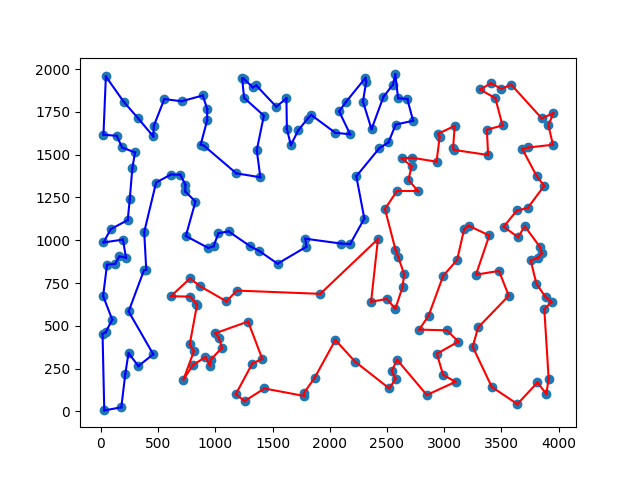
\includegraphics[width=\linewidth]{best_paths/kroA200/LNS}
        \caption{kroA200, losowy start}
    \end{minipage}
    \hfill
    \begin{minipage}[t]{0.45\textwidth}
        \centering
        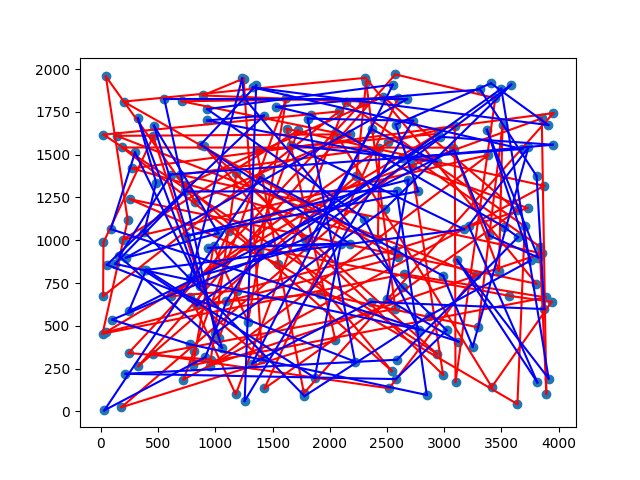
\includegraphics[width=\linewidth]{best_paths/kroB200/LNS}
        \caption{kroB200, losowy start}
    \end{minipage}\label{fig:figure2}
\end{figure}


\subsubsection{LNS bez LS}

\begin{figure}[H]
    \begin{minipage}[t]{0.45\textwidth}
        \centering
        \includegraphics[width=\linewidth]{best_paths/kroA200/LNS_bez}
        \caption{kroA200, losowy start}
    \end{minipage}
    \hfill
    \begin{minipage}[t]{0.45\textwidth}
        \centering
        \includegraphics[width=\linewidth]{best_paths/kroB200/LNS_bez}
        \caption{kroB200, losowy start}
    \end{minipage}\label{fig:figure4}
\end{figure}

\subsubsection{HAE - bazowy}

\begin{figure}[H]
    \begin{minipage}[t]{0.45\textwidth}
        \centering
        \includegraphics[width=\linewidth]{best_paths/kroA200/HAE}
        \caption{kroA200, losowy start}
    \end{minipage}
    \hfill
    \begin{minipage}[t]{0.45\textwidth}
        \centering
        \includegraphics[width=\linewidth]{best_paths/kroB200/HAE}
        \caption{kroB200, losowy start}
    \end{minipage}\label{fig:figure5}
\end{figure}

\subsubsection{HAE z mutacją}

\begin{figure}[H]
    \begin{minipage}[t]{0.45\textwidth}
        \centering
        \includegraphics[width=\linewidth]{best_paths/kroA200/HAE}
        \caption{kroA200, losowy start}
    \end{minipage}
    \hfill
    \begin{minipage}[t]{0.45\textwidth}
        \centering
        \includegraphics[width=\linewidth]{best_paths/kroB200/HAE}
        \caption{kroB200, losowy start}
    \end{minipage}\label{fig:figure6}
\end{figure}

\subsubsection{HAE z lokalnym przeszukiwaniem}

\begin{figure}[H]
    \begin{minipage}[t]{0.45\textwidth}
        \centering
        \includegraphics[width=\linewidth]{best_paths/kroA200/HAE}
        \caption{kroA200, losowy start}
    \end{minipage}
    \hfill
    \begin{minipage}[t]{0.45\textwidth}
        \centering
        \includegraphics[width=\linewidth]{best_paths/kroB200/HAE}
        \caption{kroB200, losowy start}
    \end{minipage}\label{fig:figure7}
\end{figure}


\subsubsection{HAE z mutacją i lokalnym przeszukiwaniem}

\begin{figure}[H]
    \begin{minipage}[t]{0.45\textwidth}
        \centering
        \includegraphics[width=\linewidth]{best_paths/kroA200/HAE}
        \caption{kroA200, losowy start}
    \end{minipage}
    \hfill
    \begin{minipage}[t]{0.45\textwidth}
        \centering
        \includegraphics[width=\linewidth]{best_paths/kroB200/HAE}
        \caption{kroB200, losowy start}
    \end{minipage}\label{fig:figure8}
\end{figure}


\section{Wnioski i analiza wyników}\label{sec:wnioski}

Wnioski, wnioski, wnioski, wnioski, tu serio są wnioski.
Bardzo dużo wniosków.
Patrz, jakie super wnioski!


\section{Link do repozytorium}\label{sec:link-do-repo}
Kod źródłowy w repozytorium GitHub dostępny pod linkiem: \\
\href{https://github.com/KotZPolibudy/PUT_IMO/tree/main/Lab5%20-%20Ewolucyjny}{Repozytorium}.

\end{document}
